\chapter{SegMatch}
\label{sec:segmatch}

%TODO
Intro and General Pipeline\\

Specific Pipeline, example relocalizer, onlinematcher\\

\section{Sensor Data}
\label{sec:sensordata}

Two types of sensors were used in the course of this project, rotating sensors (Velodyne) and rolling sensors (SICK). \\

Rotating sensors have a 360° view. With each rotation, they scan points along a cone originating from the sensor, resulting in a single circular scan line. This cone angle is varied by a set amount after each full rotation, with a maximum absolute angle making it so that the sensor is unable to scan the area directly above or under it. A typical rotating sensor scan is illustrated in Fig.~\ref{fig:velodyne-scan}.\\ % TODO

Rolling sensors have a 180° view, scanning towards the front and sides. The scan is flat, meaning that the points are all located on the same plane relative to the sensor’s roll angle. By varying this roll angle with every subsequent scan, the sensor can produce points at many vertical angles towards its sides. A typical rolling sensor scan is illustrated in Fig.~\ref{fig:sick-scan}.\\ % TODO

\subsection{Data Distortion}
\label{subsec:distortion}

As the sensor scans its surroundings, the robot may move and rotate. An extremum example: should the robot counter-rotate at the same angular velocity as its rotating-scanner, all points will be located on the same vertical plane in the world frame.\\

Naively mapping the full scan from sensor frame to world frame with a single affine transform will not accurately portray this effect. This is because each point was taken at a different point in time, and thus each has its own frame relative to the world frame - as the sensor was continually moving.\\

Precise knowledge of the robot’s odometry at various times during the scanning process allows to correct for distortion, by associating a different affine mapping from sensor frame to world frame to each group of points taken at a discrete rotation angle of the sensor.\\

In the case of rotating sensors, Philipp Kruesi has built the velodyne-assembler package \ref{velodyne-assembler} which corrects distortion in the aforementioned manner.\\ %TODO velodyne-assembler?

\subsection{Sensor Artifacts}
\label{subsec:artifacts}

After being corrected for distortion, sensor data contains registration patterns, as visible in Fig.~\ref{fig:velodyne-scan} (in this case, scan lines due to the rotating sensor's registration mechanics).

\section{Laser SLAM}
\label{sec:SLAM}

As single sensor scans contain registration patterns (Subsection ~\ref{subsec:artifacts}), subsequent scans should be accumulated while the robot and sensor move, in order to collect data over the whole environment. Should the scans be assembled correctly, i.e, according to the correct transform w.r.t. each other, registration patterns get progressively reduced, as the accumulated data densifies.\\

To do so, knowledge of the robot's position and orientation at each sensor aquisition time is required. When the robot odometry is not sufficiently trustworthy, the Laser SLAM algorithm allows using the sensor data to increase the odometry knowledge and improve the quality of the accumulated data.\\

\section{Segmentation}
\label{sec:segmentation}

The goal of segmentation is to delimitate clouds which should be clustered together as object representations.\\

A perfect segmentation is however not explicitely defined. Should a building be segmented into more basic components, such as walls, windows, and doors, or as single large cluster? Should a tree be clustered as a trunk with a cluster of leaves above it or as a single cluster (see Fig.~\ref{fig:hierarchical})?\\

Moosman \cite{moosmann2011unsupervised} mentions hierarchically segmenting the scene, that is not only clustering point clouds into segments, but also subsegments and subsubsegments. This hierarchy is established in order to capture those patterns that exist in real-world objects, which can be composed of smaller, simpler objects.\\

\begin{figure}
  \centering
  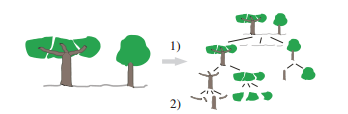
\includegraphics[width=3.2in]{images/hierarchical.png}
  \caption{Illustration of the hierarchical segmentation concept, by Moosman \cite{moosmann2011unsupervised}}
  \label{fig:hierarchical}
\end{figure}

It is useful to be aware of this concept of segment hierarchy even when using straightforward segmentation methods. By straightforward, we mean the segmentation algorithms which assign each point to at most one segment. Awareness of this hierarchy allows us to reason on where along it our segmentation algorithm works, and how that relates to the usefulness of the segments it produces.\\

For example, a specific algorithm, using a certain set of parameters, could tend to find segments which are very low in the hierarchy, i.e, smaller, less complex segments. This gives us a larger number of less unique segments, than say, running the same algorithm at a different scale.\\

By understanding this, it is easier to select the parameters which lead to optimal size, number and complexity of segments for the purposes of one's own use-case.\\

In this section, we present the main segmentation algorithms implemented and used in SegMatch. Their output and performance is compared.\\

\subsection{Euclidean Clustering}
\label{subsec:euclidean}
%TODO

Euclidean clustering is the simplest segmentation method presented here. It consists in clustering together points which fall below a certain distance threshold $\delta$ from each other.\\

It is outlined by Douillard et Al. \cite{douillard2011segmentation} as the 'Cluster-All Method' of segmentation.\\

In terms of performance, the algorithm is very fast, allowing SegMatch to perform segmentation in real-time even on the fastest moving KITTI \cite{KITTI} datasets. This is due to the algorithm's simplicity.\\

On the other hand, we often see large objects getting segmented as single clusters, and smaller objects getting clustered together simply because they happen to lie close to each other.\\

Finally, it is generally necessary to filter out the ground as it tends to connect many objects together. This can offload complexity to ground filtering in the case of complex ground geometry, but is however simple in the case of a flat city street.\\

\subsection{Difference of Normals Segmentation}
\label{subsec:DoN}
%TODO

Ioannou \cite{ioannou2012difference} presents the Difference of Normals segmentation algorithm, which aims to filter out geometrically uninteresting sections of the environment.\\

In order to do this, a difference of normals operator is defined, describing the variation in orientation with respect to scale, in the neighbouring environment. An illustration of this operator is shown in Fig.~\ref{fig:DoN}.\\

\begin{figure}
  \centering
  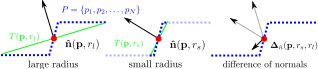
\includegraphics[width=3.2in]{images/DoN.png}
  \caption{The DoN operator according to Ioannou \cite{ioannou2012difference}}
  \label{fig:hierarchical}
\end{figure}

The average neighboring normals are first calculated at each point for neighbours which fall in a large scale radius $r_l$, then again for neighbours which fall in a small scale radius $r_s$. This process is often computationally heavy, increasingly so as the large scale increases (if nearest neighbours are not sampled).\\

For each point, a difference of normals is calculated between the average neighbour normals for the two scales. As a result, areas which are flat at both the large and small scale have a low difference of normals. Those points are filtered out, and the remaining points are clustered together if their DoN operators are similar.\\


\subsection{Optimizations}
\label{subsec:optimizations}
%TODO

D2Depth-based Segmentation
Normals from original scan

\section{Description}
\label{sec:description}
%TODO

\section{Matching}
\label{sec:matching}
%TODO

\subsection{KNN}
\label{subsec:KNN}

\subsection{Random Forests}
\label{subsec:RF}

\section{Finding Patterns}
\label{sec:filtering}

%TODO
Geometric Consistency

\section{Online Example}
\label{sec:online}

%TODO
Online segmentation strategy

\section{Results}
\label{sec:segmatch-results}
